\section[Eigenfrequenzen einer kreisförmigen Membram]{Eigenfrequenz einer kreisförmigen Membran}
\rhead{Kreisf"ormige Membran}

Eine mögliche Anwendung der Besselschen Differentialgleichung ist die Bestimmung der möglichen Eigenfrequenzen einer kreisförmigen Membran. 
Bei einem Lautsprecher ist die Membran meist an ihrem Rand eingespannt, somit ist deren Auslenkung dort immer 0. Somit können auch nur Frequenzen vorkommen, die am Rand der Membran eine Nullstelle haben. Wir erhalten somit ein Randwertproblem
\index{Randwertproblem}
\begin{equation}
r^2 R''(r) + r R'(r) + (-\mu r^2 - n^2)R(r) = 0
\label{eq:dglmitmu}
\end{equation}
mit 
\[
R(\rho) = 0,
\]
wobei $\rho$ der Radius der Membran ist.
Wie wir im Abschnitt~\ref{kreis:teil2} gesehen haben, ist das $n$ frei wählbar als Index der entsprechenden Bessel-Funktion, somit ist noch das $\mu$ zu bestimmen. 
Dazu definieren wir die Funktion
\[
F(r) = J_n \biggl(\frac{r}{a} \biggr),
\]
mit den Ableitungen
\[
F'(r) = \frac{r}{a} J_n \biggl(\frac{r}{a} \biggr)
\]
und 
\[
F''(r) = \frac{r^2}{a^2} J_n \biggl(\frac{r}{a} \biggr).
\]
Setzen wir dies in die Differentialgleichung \refeq{eq:dglmitmu} ein, erhalten wir
\begin{equation}
\frac{r^2}{a^2}J_n''\biggl(\frac{r}{a} \biggr) +
\frac{r}{a}J_n'\biggl(\frac{r}{a} \biggr) +
\biggl(\frac{r^2}{a^2} - k^2\biggr)J_n\biggl(\frac{r}{a}\biggr) = 0.
\label{eq:dglmitfaktor}
\end{equation}
Wir sehen, dass $\frac{1}{a^2}=-\mu$ entspricht.
Für $J_0(r)$ wissen wir, dass die Nullstelle der Grundfrequenz bei $\rho$ liegen muss, somit gilt
\[
\frac{\rho}{a} = r_0.
\]
Für den  Zusammenhang zwischen der Frequenz und dem $\mu$ betrachten wir die Zeitgleichung in \refeq{eq:separiertegleichung}. Formt man diese Gleichung nach $T''(t)$ um, so erhält man 
\[
\frac{1}{c^2} T''(t) = \mu T(t).
\]
Die Lösung dieser Gleichung sind bekanntlich $\sin(\omega t)$ und $\cos(\omega t)$, welche mittels eulerscher Formel als $e^{i\omega t}$ geschrieben werden können.
Setzen wir dies in die Gleichung ein, erhalten wir
\[
\frac{1}{c^2}(i\omega)^2 e^{i\omega t} = \mu e^{i\omega t}
\]
Da der Faktor $\frac{1}{c^2}$ für die Geschwindigkeit der Welle steht, kann er für die Betrachtung der Frequenz vernachlässigt werden. Wir erhalten somit die Gleichung
$
-\omega^2 e^{i\omega t} = \mu e^{i\omega t}.
$
Lösen wir diese Gleichung nach $\mu$ auf, so erhalten wir
$
\mu = -\omega^2
$.
Wie wir bei Gleichung \refeq{eq:dglmitfaktor} gesehen haben, entspricht gilt $\mu = -\frac{1}{a^2}$. Somit gilt die Beziehung
\[
\frac{1}{a^2} = \frac{r_0^2}{\rho^2} = -\omega^2
\Leftrightarrow
\frac{r_0}{\rho} = i\omega.
\]
Um nun die Frequenzen zu finden, welche auf einer Membran mit bestimmten Radius vorkommen, können wir die Gleichung
\[
J_n(ar) = 0
\]
aufstellen.

Da für diese Gleichung für mehrere Werte sowie auch für mehrere Funktionen erfüllt ist, lässt man diese am besten durch einen Computer berechnen. Die meisten Programme wie z.B. Mathematica oder Matlab haben eingebaute Funktionen um Nullstellen von Besselfunktionen zu berechnen.
Folgend die ersten fünf Nullstellen der ersten sechs Besselschen Funtionen:
\begin{center}
\begin{tabular}{>{$}c<{$}|>{$}c<{$}>{$}c<{$}>{$}c<{$}>{$}c<{$}>{$}c<{$}>{$}c<{$}}
   & J_0(r) & J_1(r) & J_2(r) & J_3(r) & J_4(r) & J_5(r) \\
\hline
 1 & \phantom{0}2.4048 & \phantom{0}3.8317 & \phantom{0}5.1356 & \phantom{0}6.3802 & \phantom{ }7.5883 & \phantom{ }8.7715 \\
 2 & \phantom{0}5.5201 & \phantom{0}7.0156 & \phantom{0}8.4172 & \phantom{0}9.7610 & 11.0647 & 12.3386 \\
 3 & \phantom{0}8.6537 & 10.1735 & 11.6198 & 13.0152 & 14.3725 & 15.7002 \\
 4 & 11.7915 & 13.3237 & 14.7960 & 16.2235 & 17.6160 & 18.9801 \\
 5 & 14.9309 & 16.4706 & 17.9598 & 19.4094 & 20.8269 & 22.2178 \\
\end{tabular}
\end{center}
Wie aus der Tabelle zu entnehmen ist, kommen nicht nur ganzzahlige Vielfache vor. Somit ist das Obertonspektrum eines Lautsprechers nicht rein harmonisch.
Zur Veranschaulichung wie sich die besselschen Funktionen auf die Schwingungen einer Membran auswirken, sind folgend jeweils die ersten drei Schwingungen der mit Radialfunktionen $J_0(r)$, $J_1(r)$ und $J_2(r)$ geplottet.
\begin{figure}
        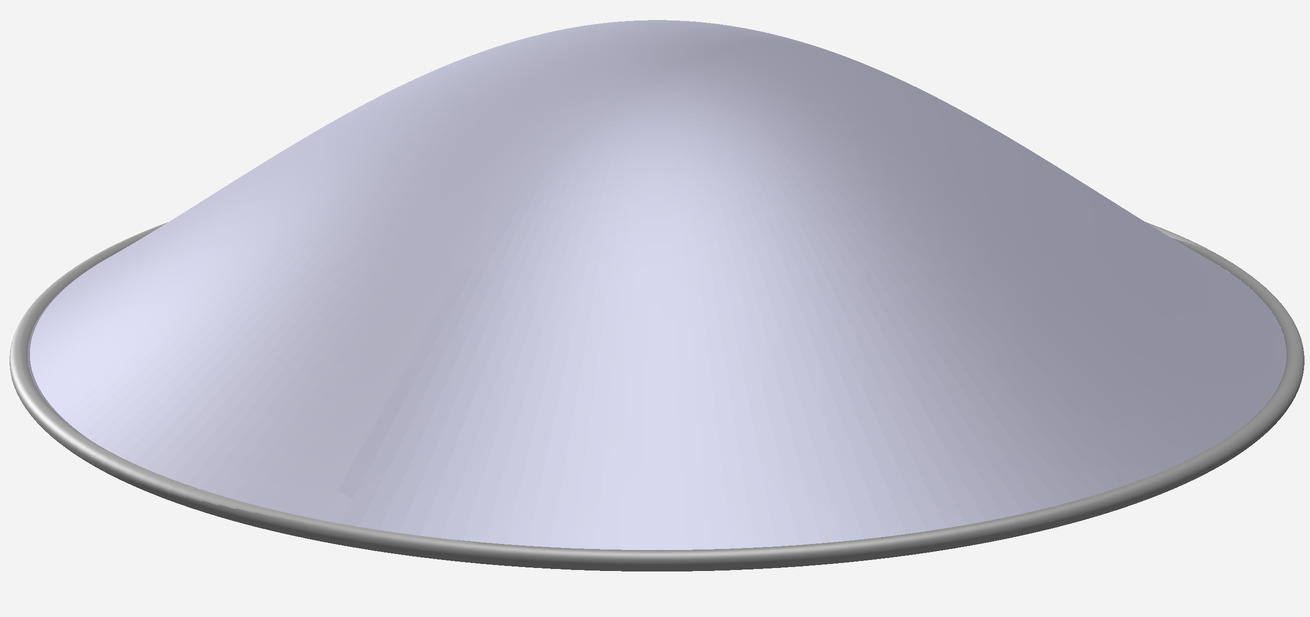
\includegraphics[width=0.33\hsize]{./kreis/membran/circle-1-0.jpg}
        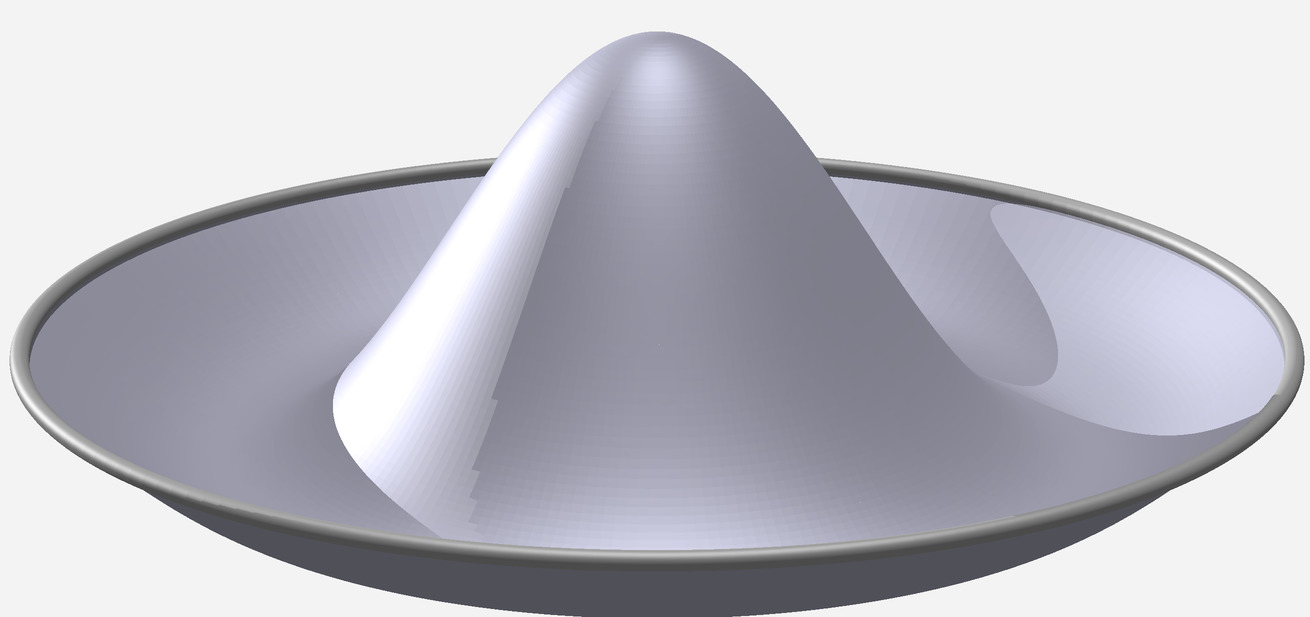
\includegraphics[width=0.33\hsize]{./kreis/membran/circle-2-0.jpg}
        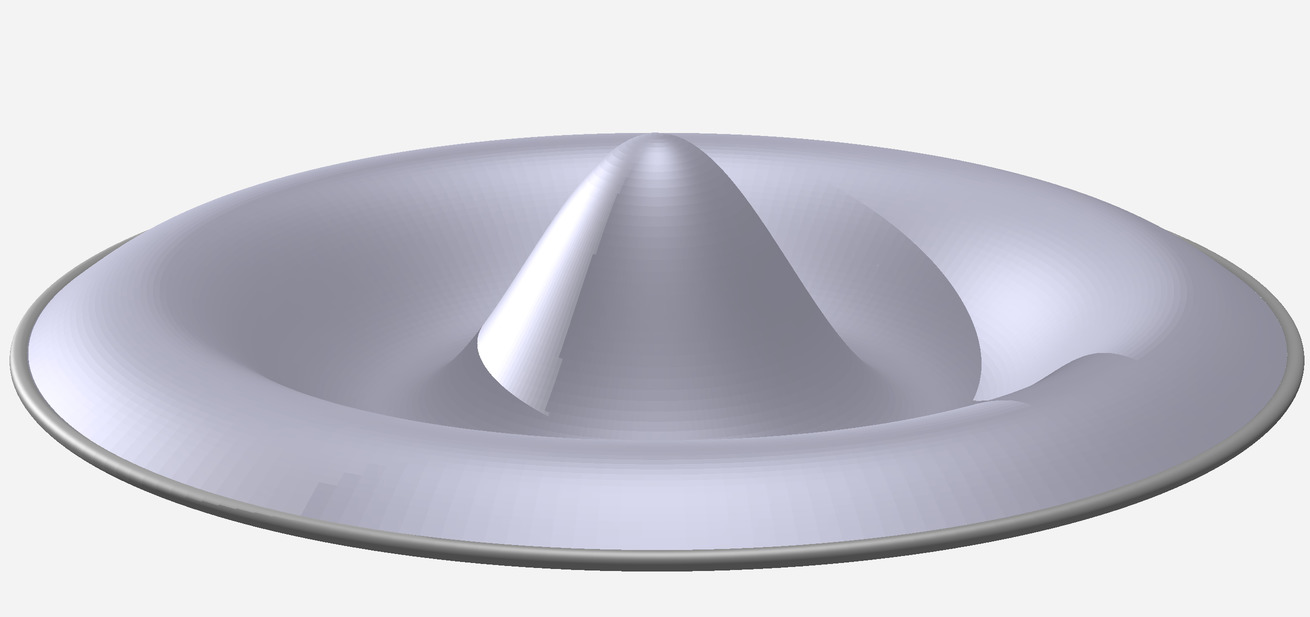
\includegraphics[width=0.33\hsize]{./kreis/membran/circle-3-0.jpg}
        \caption{Schwingungen(Grundschwingung sowie 1. und 2. Oberschwingung) mit Radialfunktion $J_0(r)$}
        \label{fig:membranj0}
\bigskip
%\end{figure}
%\begin{figure}
        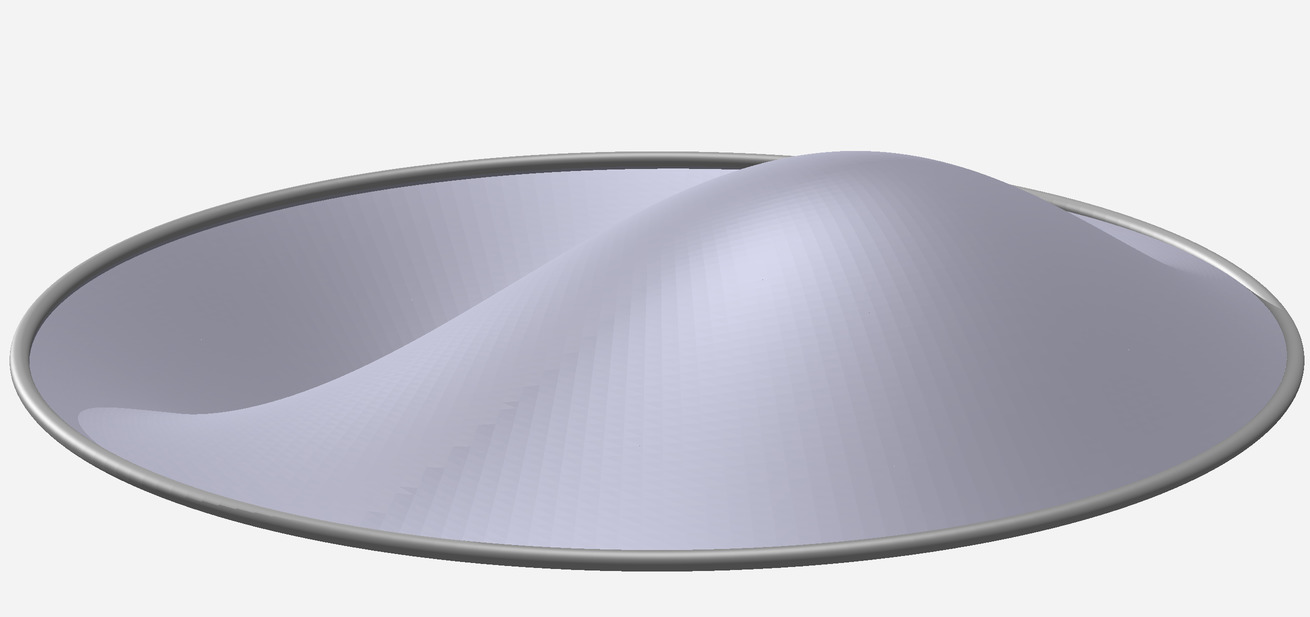
\includegraphics[width=0.33\hsize]{./kreis/membran/circle-1-1.jpg}
        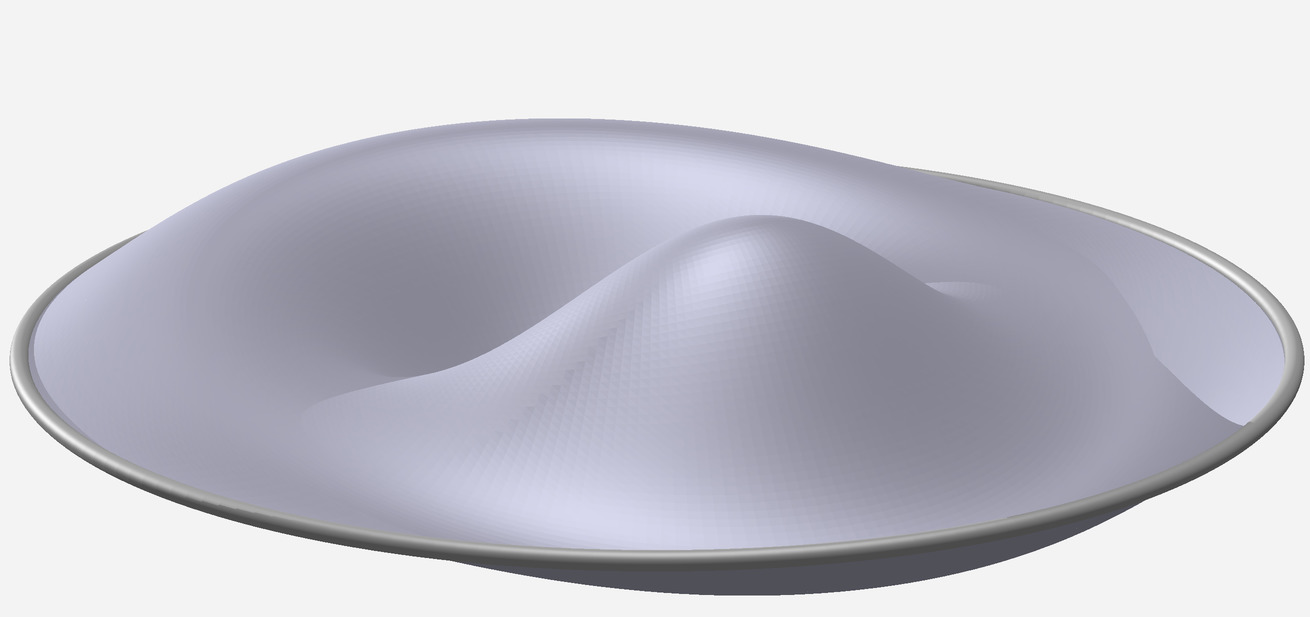
\includegraphics[width=0.33\hsize]{./kreis/membran/circle-2-1.jpg}
        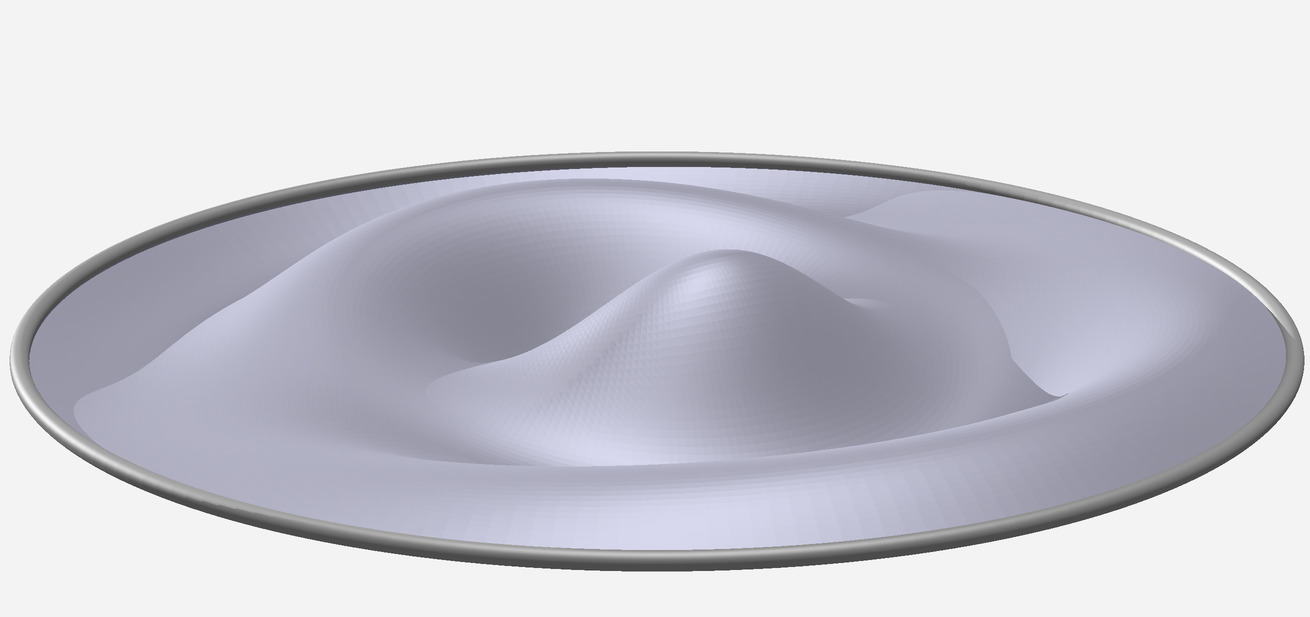
\includegraphics[width=0.33\hsize]{./kreis/membran/circle-3-1.jpg}
        \caption{Schwingungen(Grundschwingung sowie 1. und 2. Oberschwingung) mit Radialfunktion $J_1(r)$}
        \label{fig:membranj1}
\bigskip
%\end{figure}
%\begin{figure}
        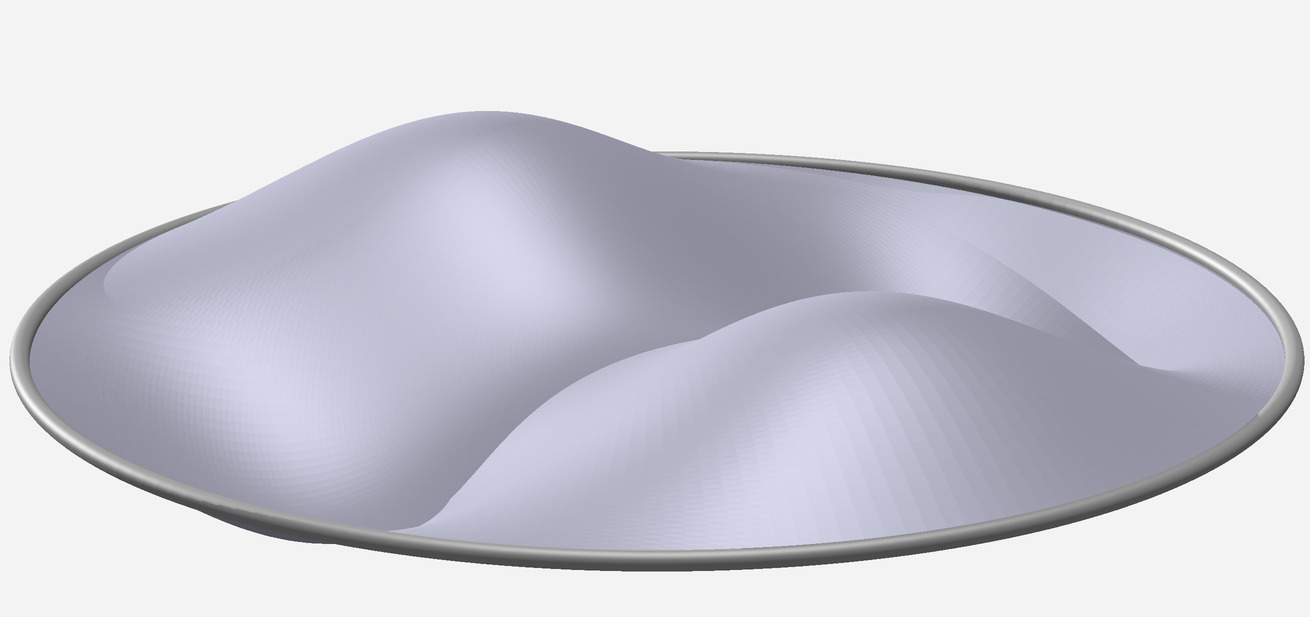
\includegraphics[width=0.33\hsize]{./kreis/membran/circle-1-2.jpg}
        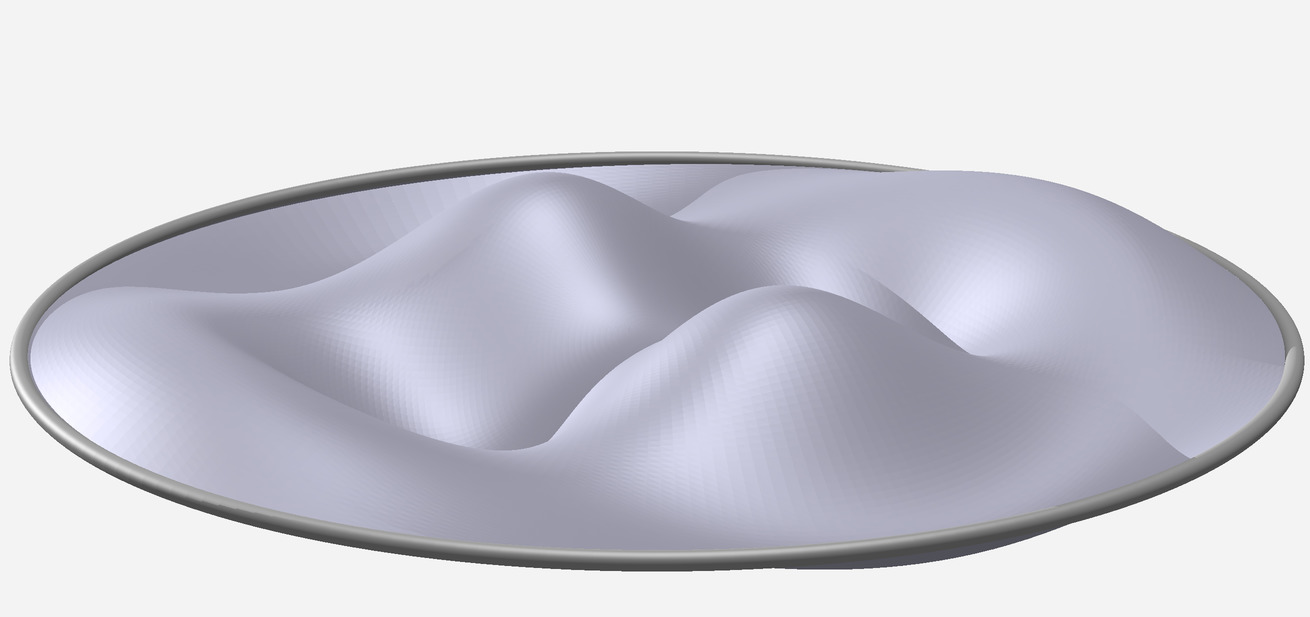
\includegraphics[width=0.33\hsize]{./kreis/membran/circle-2-2.jpg}
        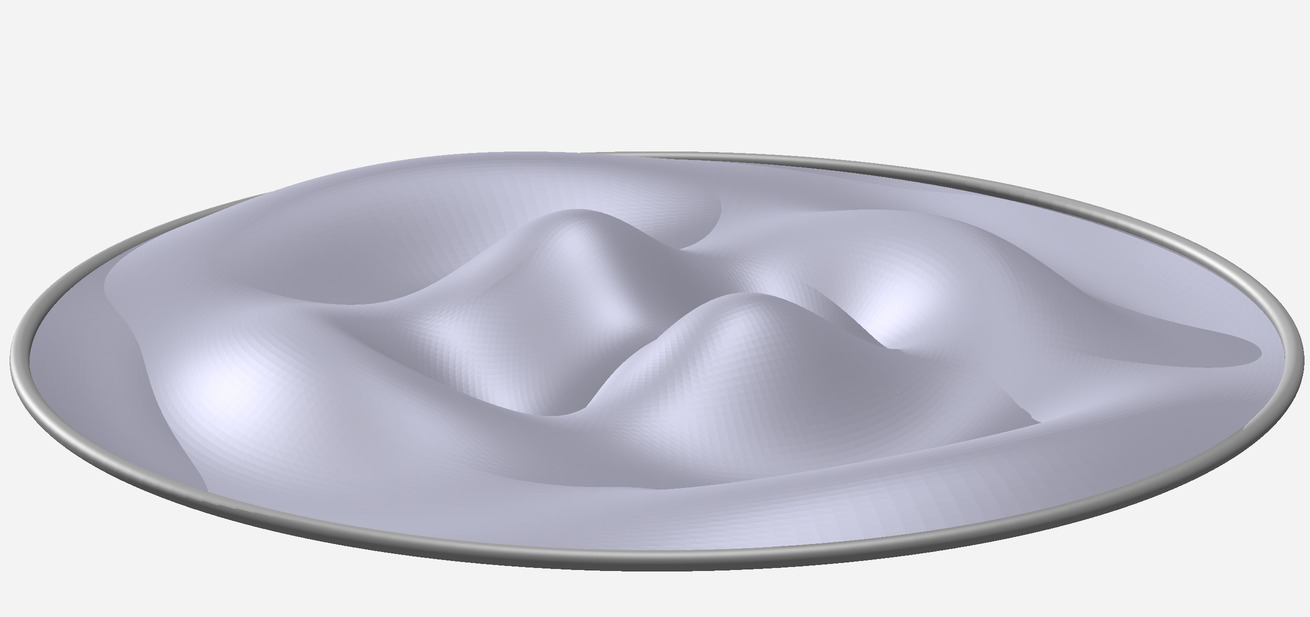
\includegraphics[width=0.33\hsize]{./kreis/membran/circle-3-2.jpg}
        \caption{Schwingungen(Grundschwingung sowie 1. und 2. Oberschwingung) mit Radialfunktion $J_2(r)$}
        \label{fig:membranj2}
\end{figure}
Wie aus der Abbildung \ref{fig:membranj0} zu erkennen ist befinden sich alle Nullstellen auf konzentrischen Kreisen um den Mittelpunkt mit der ersten Nullstelle am Rand.

Bei den höheren Besselfunktionen wie in Abbildung~\ref{fig:membranj1} und Abbildung~\ref{fig:membranj2} befindet sich jeweils eine Nullstelle im Zentrum der Membran. Dies ist nicht weiter erstaunlich, denn die Besselfunktionen grösser $J_0$ haben bei 0 eine Nullstelle. 
